% Options for packages loaded elsewhere
% Options for packages loaded elsewhere
\PassOptionsToPackage{unicode}{hyperref}
\PassOptionsToPackage{hyphens}{url}
%
\documentclass[
  english,
  russian,
  12pt,
  a4paper,
  DIV=11,
  numbers=noendperiod]{scrreprt}
\usepackage{xcolor}
\usepackage{amsmath,amssymb}
\setcounter{secnumdepth}{5}
\usepackage{iftex}
\ifPDFTeX
  \usepackage[T1]{fontenc}
  \usepackage[utf8]{inputenc}
  \usepackage{textcomp} % provide euro and other symbols
\else % if luatex or xetex
  \usepackage{unicode-math} % this also loads fontspec
  \defaultfontfeatures{Scale=MatchLowercase}
  \defaultfontfeatures[\rmfamily]{Ligatures=TeX,Scale=1}
\fi
\usepackage{lmodern}
\ifPDFTeX\else
  % xetex/luatex font selection
\fi
% Use upquote if available, for straight quotes in verbatim environments
\IfFileExists{upquote.sty}{\usepackage{upquote}}{}
\IfFileExists{microtype.sty}{% use microtype if available
  \usepackage[]{microtype}
  \UseMicrotypeSet[protrusion]{basicmath} % disable protrusion for tt fonts
}{}
\usepackage{setspace}
% Make \paragraph and \subparagraph free-standing
\makeatletter
\ifx\paragraph\undefined\else
  \let\oldparagraph\paragraph
  \renewcommand{\paragraph}{
    \@ifstar
      \xxxParagraphStar
      \xxxParagraphNoStar
  }
  \newcommand{\xxxParagraphStar}[1]{\oldparagraph*{#1}\mbox{}}
  \newcommand{\xxxParagraphNoStar}[1]{\oldparagraph{#1}\mbox{}}
\fi
\ifx\subparagraph\undefined\else
  \let\oldsubparagraph\subparagraph
  \renewcommand{\subparagraph}{
    \@ifstar
      \xxxSubParagraphStar
      \xxxSubParagraphNoStar
  }
  \newcommand{\xxxSubParagraphStar}[1]{\oldsubparagraph*{#1}\mbox{}}
  \newcommand{\xxxSubParagraphNoStar}[1]{\oldsubparagraph{#1}\mbox{}}
\fi
\makeatother


\usepackage{longtable,booktabs,array}
\usepackage{calc} % for calculating minipage widths
% Correct order of tables after \paragraph or \subparagraph
\usepackage{etoolbox}
\makeatletter
\patchcmd\longtable{\par}{\if@noskipsec\mbox{}\fi\par}{}{}
\makeatother
% Allow footnotes in longtable head/foot
\IfFileExists{footnotehyper.sty}{\usepackage{footnotehyper}}{\usepackage{footnote}}
\makesavenoteenv{longtable}
\usepackage{graphicx}
\makeatletter
\newsavebox\pandoc@box
\newcommand*\pandocbounded[1]{% scales image to fit in text height/width
  \sbox\pandoc@box{#1}%
  \Gscale@div\@tempa{\textheight}{\dimexpr\ht\pandoc@box+\dp\pandoc@box\relax}%
  \Gscale@div\@tempb{\linewidth}{\wd\pandoc@box}%
  \ifdim\@tempb\p@<\@tempa\p@\let\@tempa\@tempb\fi% select the smaller of both
  \ifdim\@tempa\p@<\p@\scalebox{\@tempa}{\usebox\pandoc@box}%
  \else\usebox{\pandoc@box}%
  \fi%
}
% Set default figure placement to htbp
\def\fps@figure{htbp}
\makeatother



\ifLuaTeX
\usepackage[bidi=basic,provide=*]{babel}
\else
\usepackage[bidi=default,provide=*]{babel}
\fi
% get rid of language-specific shorthands (see #6817):
\let\LanguageShortHands\languageshorthands
\def\languageshorthands#1{}


\setlength{\emergencystretch}{3em} % prevent overfull lines

\providecommand{\tightlist}{%
  \setlength{\itemsep}{0pt}\setlength{\parskip}{0pt}}



 
\usepackage[backend=biber,langhook=extras,autolang=other*]{biblatex}
\addbibresource{bib/cite.bib}

\usepackage[]{csquotes}

\usepackage{indentfirst}
\usepackage{float}
\floatplacement{figure}{H}
\IfFileExists{plex-otf.sty}{
  %% Full TeXlive
  \IfPackageAtLeastTF{plex-otf.sty}{2024-12-06}{
    \usepackage[math,RM={Scale=0.94},SS={Scale=0.94},SScon={Scale=0.94},TT={Scale=MatchLowercase,FakeStretch=0.9},DefaultFeatures={Ligatures=Common}]{plex-otf}
  }{
    \usepackage[RM={Scale=0.94},SS={Scale=0.94},SScon={Scale=0.94},TT={Scale=MatchLowercase,FakeStretch=0.9},DefaultFeatures={Ligatures=Common}]{plex-otf}
  }
}{
  %% TinyTeX
  \usepackage{libertine}
}
\KOMAoption{captions}{tableheading}
\makeatletter
\@ifpackageloaded{caption}{}{\usepackage{caption}}
\AtBeginDocument{%
\ifdefined\contentsname
  \renewcommand*\contentsname{Содержание}
\else
  \newcommand\contentsname{Содержание}
\fi
\ifdefined\listfigurename
  \renewcommand*\listfigurename{Список Иллюстраций}
\else
  \newcommand\listfigurename{Список Иллюстраций}
\fi
\ifdefined\listtablename
  \renewcommand*\listtablename{Список Таблиц}
\else
  \newcommand\listtablename{Список Таблиц}
\fi
\ifdefined\figurename
  \renewcommand*\figurename{Рисунок}
\else
  \newcommand\figurename{Рисунок}
\fi
\ifdefined\tablename
  \renewcommand*\tablename{Таблица}
\else
  \newcommand\tablename{Таблица}
\fi
}
\@ifpackageloaded{float}{}{\usepackage{float}}
\floatstyle{ruled}
\@ifundefined{c@chapter}{\newfloat{codelisting}{h}{lop}}{\newfloat{codelisting}{h}{lop}[chapter]}
\floatname{codelisting}{Список}
\newcommand*\listoflistings{\listof{codelisting}{Список Каталогов}}
\makeatother
\makeatletter
\makeatother
\makeatletter
\@ifpackageloaded{caption}{}{\usepackage{caption}}
\@ifpackageloaded{subcaption}{}{\usepackage{subcaption}}
\makeatother
\usepackage{bookmark}
\IfFileExists{xurl.sty}{\usepackage{xurl}}{} % add URL line breaks if available
\urlstyle{same}
\hypersetup{
  pdftitle={ЛАБОРАТОРНАЯ РАБОТА Nº8},
  pdfauthor={Хамза хуссен},
  pdflang={ru-RU},
  hidelinks,
  pdfcreator={LaTeX via pandoc}}


\title{ЛАБОРАТОРНАЯ РАБОТА Nº8}
\usepackage{etoolbox}
\makeatletter
\providecommand{\subtitle}[1]{% add subtitle to \maketitle
  \apptocmd{\@title}{\par {\large #1 \par}}{}{}
}
\makeatother
\subtitle{Целочисленная арифметика многократной точности}
\author{Хамза хуссен}
\date{}
\begin{document}
\maketitle

\renewcommand*\contentsname{Содержание}
{
\setcounter{tocdepth}{1}
\tableofcontents
}

\setstretch{1.5}
\chapter{Цель
работы}\label{ux446ux435ux43bux44c-ux440ux430ux431ux43eux442ux44b}

Реализация алгоритмов многократной точности для целочисленной
арифметики.

\chapter{Задание}\label{ux437ux430ux434ux430ux43dux438ux435}

\begin{enumerate}
\def\labelenumi{\arabic{enumi}.}
\item
  Реализовать алгоритм сложения неотрицательных целых чисел.
\item
  Реализовать алгоритм вычитания неотрицательных целых чисел.
\item
  Реализовать алгоритм умножения неотрицательных целых чисел столбиком.
\item
  Реализовать алгоритм умножения методом быстрого столбика.
\item
  Реализовать алгоритм деления неотрицательных целых чисел.
\end{enumerate}

\chapter{Теоретическое
введение}\label{ux442ux435ux43eux440ux435ux442ux438ux447ux435ux441ux43aux43eux435-ux432ux432ux435ux434ux435ux43dux438ux435}

Рассмотрим алгоритмы для выполнения арифметических операций с большими
целыми числами. Будем считать, что число записано в b - ичной системе
счисления, \(b - натуральное число, b ≥ 2\). Натуральное -разрядное
число будем записывать в виде: \(u = u_1 u_2 \ldots u_n\)

\section{Алгоритм сложения неотрицательных целых
чисел}\label{ux430ux43bux433ux43eux440ux438ux442ux43c-ux441ux43bux43eux436ux435ux43dux438ux44f-ux43dux435ux43eux442ux440ux438ux446ux430ux442ux435ux43bux44cux43dux44bux445-ux446ux435ux43bux44bux445-ux447ux438ux441ux435ux43b}

*Вход. Два неотрицательных числа \(u = u_1 u_2 \ldots u_n\) и
\(v = v_1 v_2 \ldots v_n\); разрядность чисел \(n\); основание системы
счисления \(b\).

*Выход. Сумма \(w = w_0 w_1 \ldots w_n\), где \(w_0\) - цифра переноса,
всегда равная \(0\) либо \(1\).

\begin{enumerate}
\def\labelenumi{\arabic{enumi}.}
\tightlist
\item
  Присвоить \(j = n, k = 0\) (\emph{\(j\) идет по разрядам, \(k\) следит
  за переносом}).
\item
  Присвоить \(w_j = (u_j + v_j + k) \pmod{b}\), где
  \(k = \left[ \frac{u_j + v_j + k}{b} \right]\).
\item
  Присвоить \(j = j - 1\). Если \(j > 0\), то возвращаемся на шаг 2;
  если \(j = 0\), то присвоить \(w_0 = k\) и результат: \(w\).
\end{enumerate}

\section{Алгоритм вычитания неотрицательных целых
чисел}\label{ux430ux43bux433ux43eux440ux438ux442ux43c-ux432ux44bux447ux438ux442ux430ux43dux438ux44f-ux43dux435ux43eux442ux440ux438ux446ux430ux442ux435ux43bux44cux43dux44bux445-ux446ux435ux43bux44bux445-ux447ux438ux441ux435ux43b}

*Вход. Два неотрицательных числа \(u = u_1 u_2 \ldots u_n\) и
\(v = v_1 v_2 \ldots v_n\), \(u > v\); разрядность чисел \(n\);
основание системы счисления \(b\).

*Выход. Разность \(w = w_0 w_1 \ldots w_n = u - v\).

\begin{enumerate}
\def\labelenumi{\arabic{enumi}.}
\tightlist
\item
  Присвоить \(j = n, k = 0\) (\(k\) -- заём из старшего разряда).
\item
  Присвоить \(w_j = (u_j - v_j + k) \pmod{b}\);
  \(k = \left[ \frac{u_j - v_j + k}{b} \right]\).
\item
  Присвоить \(j = j - 1\). Если \(j > 0\), то возвращаемся на шаг 2;
  если \(j = 0\), то результат: \(w\).
\end{enumerate}

\section{Алгоритм умножения неотрицательных целых чисел
столбиком}\label{ux430ux43bux433ux43eux440ux438ux442ux43c-ux443ux43cux43dux43eux436ux435ux43dux438ux44f-ux43dux435ux43eux442ux440ux438ux446ux430ux442ux435ux43bux44cux43dux44bux445-ux446ux435ux43bux44bux445-ux447ux438ux441ux435ux43b-ux441ux442ux43eux43bux431ux438ux43aux43eux43c}

*Вход. Числа \(u = u_1 u_2 \ldots u_n\), \(v = v_1 v_2 \ldots v_m\);
основание системы счисления \(b\).

*Выход. Произведение \(w = uv = w_1 w_2 \ldots w_{m+n}\).

\begin{enumerate}
\def\labelenumi{\arabic{enumi}.}
\tightlist
\item
  Выполнить присвоения:
  \(w_{m+1} = 0, w_{m+2} = 0, \ldots, w_{m+n} = 0, j = m\) (\emph{\(j\)
  перемещается по номерам разрядов числа \(v\) от младших к старшим}).
\item
  Если \(v_j = 0\), то присвоить \(w_j = 0\) и перейти на шаг 6.
\item
  Присвоить \(i = n, k = 0\) (\emph{значение \(i\) идет по номерам
  разрядов числа \(u\), \(k\) отвечает за перенос}).
\item
  Присвоить
  \(t = u_i \cdot v_j + w_{i+j} + k, w_{i+j} = t \pmod{b}, k = \left[ \frac{t}{b} \right]\).
\item
  Присвоить \(i = i - 1\). Если \(i > 0\), то возвращаемся на шаг 4,
  иначе присвоить \(w_j = k\).
\item
  Присвоить \(j = j - 1\). Если \(j > 0\), то вернуться на шаг 2. Если
  \(j = 0\), то результат: \(w\).
\end{enumerate}

\section{Алгоритм умножения методом быстрого
столбика}\label{ux430ux43bux433ux43eux440ux438ux442ux43c-ux443ux43cux43dux43eux436ux435ux43dux438ux44f-ux43cux435ux442ux43eux434ux43eux43c-ux431ux44bux441ux442ux440ux43eux433ux43e-ux441ux442ux43eux43bux431ux438ux43aux430}

*Вход. Числа \(u = u_1 u_2 \ldots u_n\), \(v = v_1 v_2 \ldots v_m\);
основание системы счисления \(b\).

*Выход. Произведение \(w = uv = w_1 w_2 \ldots w_{m+n}\).

\begin{enumerate}
\def\labelenumi{\arabic{enumi}.}
\tightlist
\item
  Присвоить \(t = 0\).
\item
  Для \(s\) от \(0\) до \(m + n - 1\) с шагом 1 выполнить шаги 3 и 4.
\item
  Для \(i\) от \(0\) до \(s\) с шагом 1 выполнить присвоение
  \(t~=~t~+~u_{n - i}~\cdot~v_{m - s + i}\).
\item
  Присвоить
  \(w_{m + n - s} = t \pmod{b}, t = \left[ \frac{t}{b} \right]\).
  Результат: \(w\).
\end{enumerate}

\section{Алгоритм деления неотрицательных целых
чисел}\label{ux430ux43bux433ux43eux440ux438ux442ux43c-ux434ux435ux43bux435ux43dux438ux44f-ux43dux435ux43eux442ux440ux438ux446ux430ux442ux435ux43bux44cux43dux44bux445-ux446ux435ux43bux44bux445-ux447ux438ux441ux435ux43b}

*Вход. Числа \(u = u_n \ldots u_1 u_0\),
\(v = v_t \ldots v_1 v_0, n \ge t \ge 1, v_t \ne 0\).

*Выход. Частное \(q = q_{n-t} \ldots q_0\), остаток
\(r = r_t \ldots r_0\).

\begin{enumerate}
\def\labelenumi{\arabic{enumi}.}
\tightlist
\item
  Для \(j\) от \(0\) до \(n - t\) присвоить \(q_j = 0\).
\item
  Пока \(u \ge v b^{n - t}\), выполнять:
  \(q_{n - t} = q_{n - t} + 1, u = u - v b^{n - t}\).
\item
  Для \(i = n, n - 1, \ldots, t + 1\) выполнять пункты 3.1 -- 3.4: 3.1.
  если \(u_i \ge v_t\), то присвоить \(q_{i - t - 1} = b - 1\), иначе
  присвоить \(q_{i - t - 1} = \frac{u_i b + u_{i - 1}}{v_t}\). 3.2. пока
  \(q_{i - t - 1} (v_t b + v_{t - 1}) > u_i b^2 + u_{i - 1} b + u_{i - 2}\)
  выполнять \(q_{i - t - 1} = q_{i - t - 1} - 1\). 3.3. присвоить
  \(u = u - q_{i - t - 1} b^{i - t - 1} v\). 3.4. если \(u < 0\), то
  присвоить \(u = u + v b^{i - t - 1}\),
  \(q_{i - t - 1}~=~q_{i - t - 1}~-~1\).
\item
  \(r = u\). Результат: \(q\) и \(r\).
\end{enumerate}

\chapter{Выполнение лабораторной
работы}\label{ux432ux44bux43fux43eux43bux43dux435ux43dux438ux435-ux43bux430ux431ux43eux440ux430ux442ux43eux440ux43dux43eux439-ux440ux430ux431ux43eux442ux44b}

\section{Реализация Алгоритма сложения неотрицательных целых
чисел}\label{ux440ux435ux430ux43bux438ux437ux430ux446ux438ux44f-ux430ux43bux433ux43eux440ux438ux442ux43cux430-ux441ux43bux43eux436ux435ux43dux438ux44f-ux43dux435ux43eux442ux440ux438ux446ux430ux442ux435ux43bux44cux43dux44bux445-ux446ux435ux43bux44bux445-ux447ux438ux441ux435ux43b}

\begin{figure}[H]

{\centering \pandocbounded{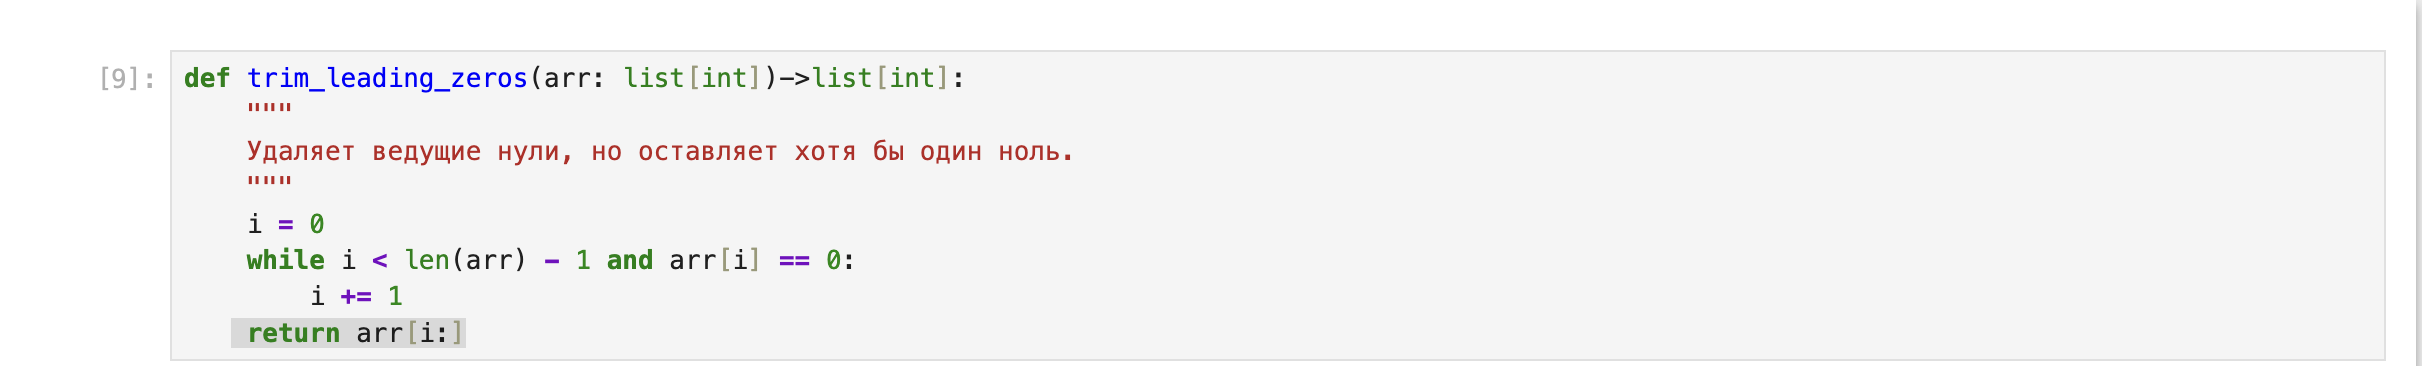
\includegraphics[keepaspectratio]{./image/img_15.png}}

}

\caption{trim\_leading\_zeros}

\end{figure}%

\begin{figure}[H]

{\centering \pandocbounded{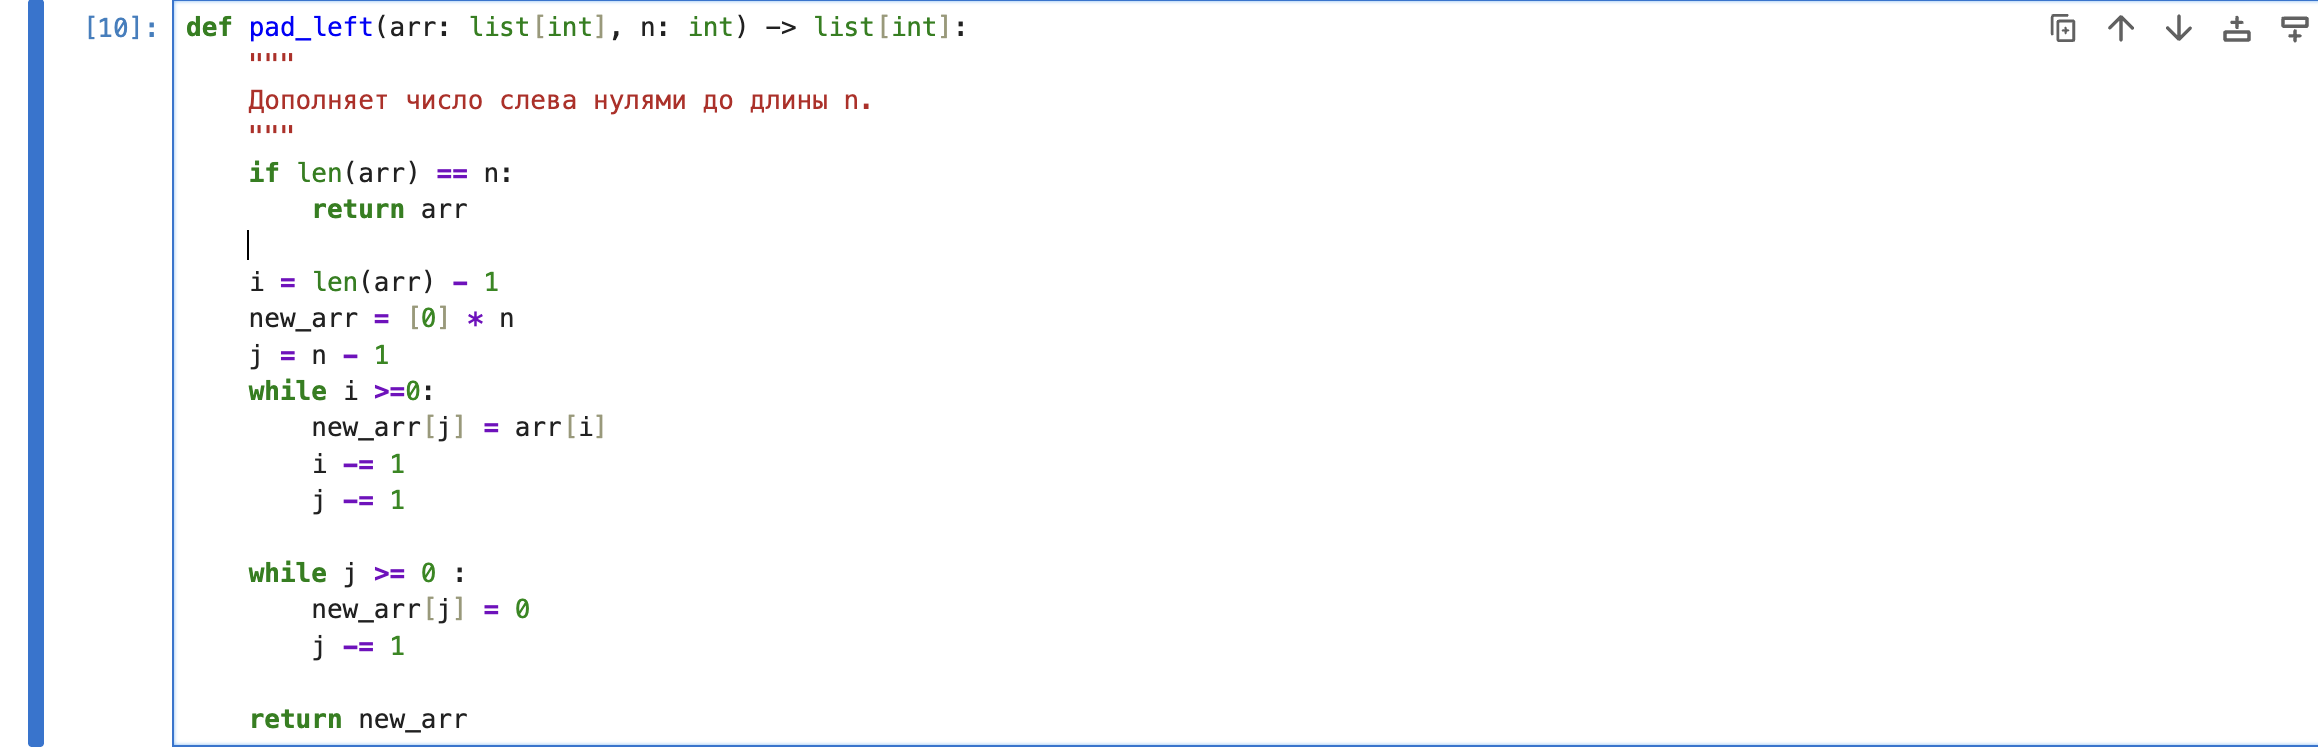
\includegraphics[keepaspectratio]{./image/img_14.png}}

}

\caption{pad\_left}

\end{figure}%

\begin{figure}[H]

{\centering \pandocbounded{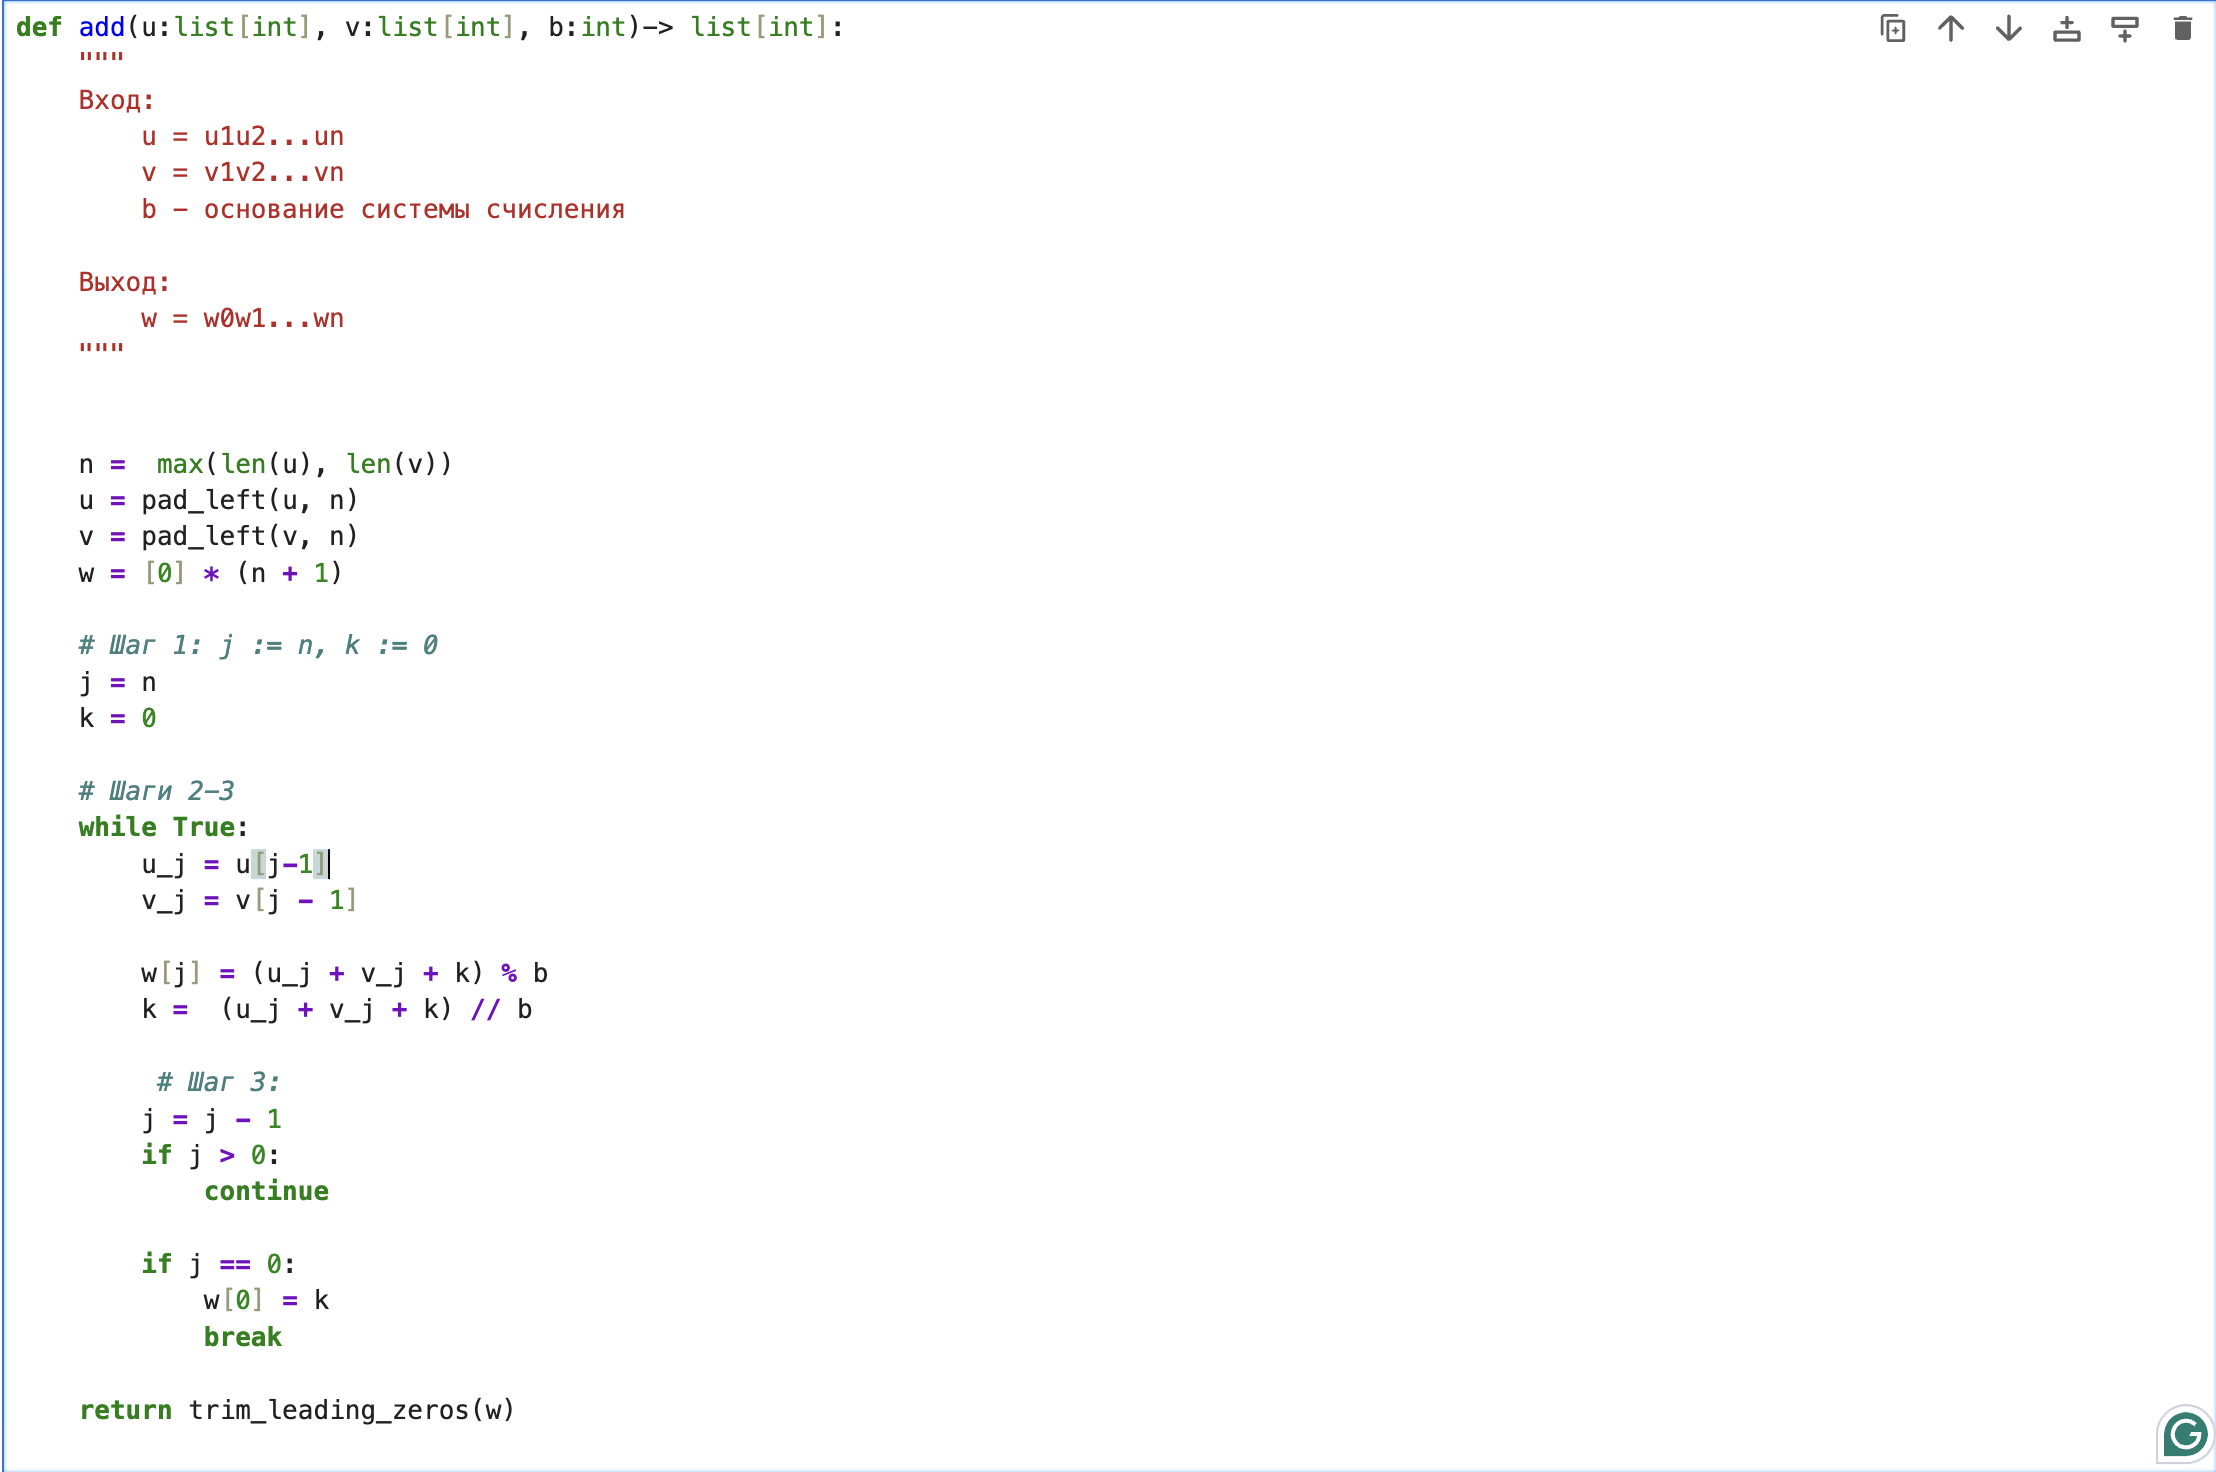
\includegraphics[keepaspectratio]{./image/img_13.png}}

}

\caption{add}

\end{figure}%

\begin{figure}[H]

{\centering \pandocbounded{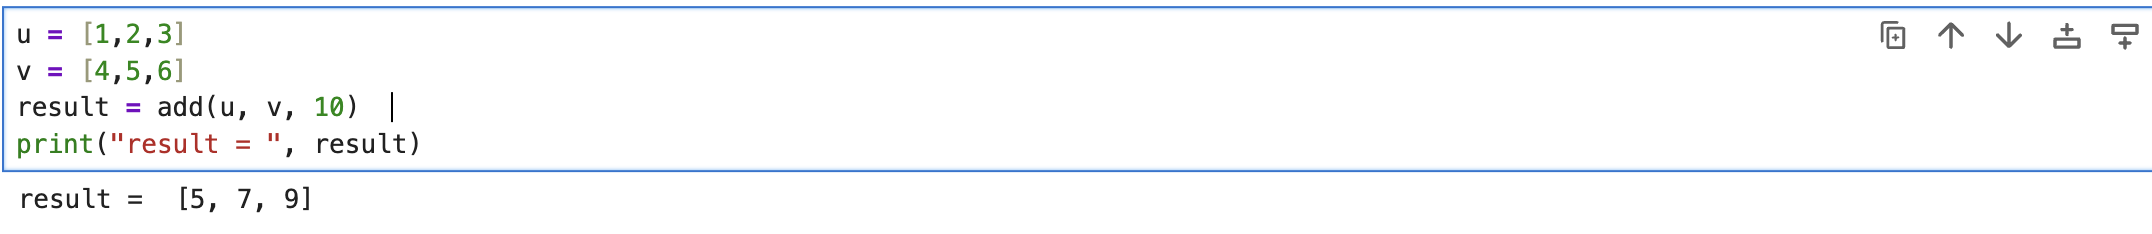
\includegraphics[keepaspectratio]{./image/img_12.png}}

}

\caption{result}

\end{figure}%

\section{Реализация Алгоритма вычитания неотрицательных целых
чисел}\label{ux440ux435ux430ux43bux438ux437ux430ux446ux438ux44f-ux430ux43bux433ux43eux440ux438ux442ux43cux430-ux432ux44bux447ux438ux442ux430ux43dux438ux44f-ux43dux435ux43eux442ux440ux438ux446ux430ux442ux435ux43bux44cux43dux44bux445-ux446ux435ux43bux44bux445-ux447ux438ux441ux435ux43b}

\begin{figure}[H]

{\centering \pandocbounded{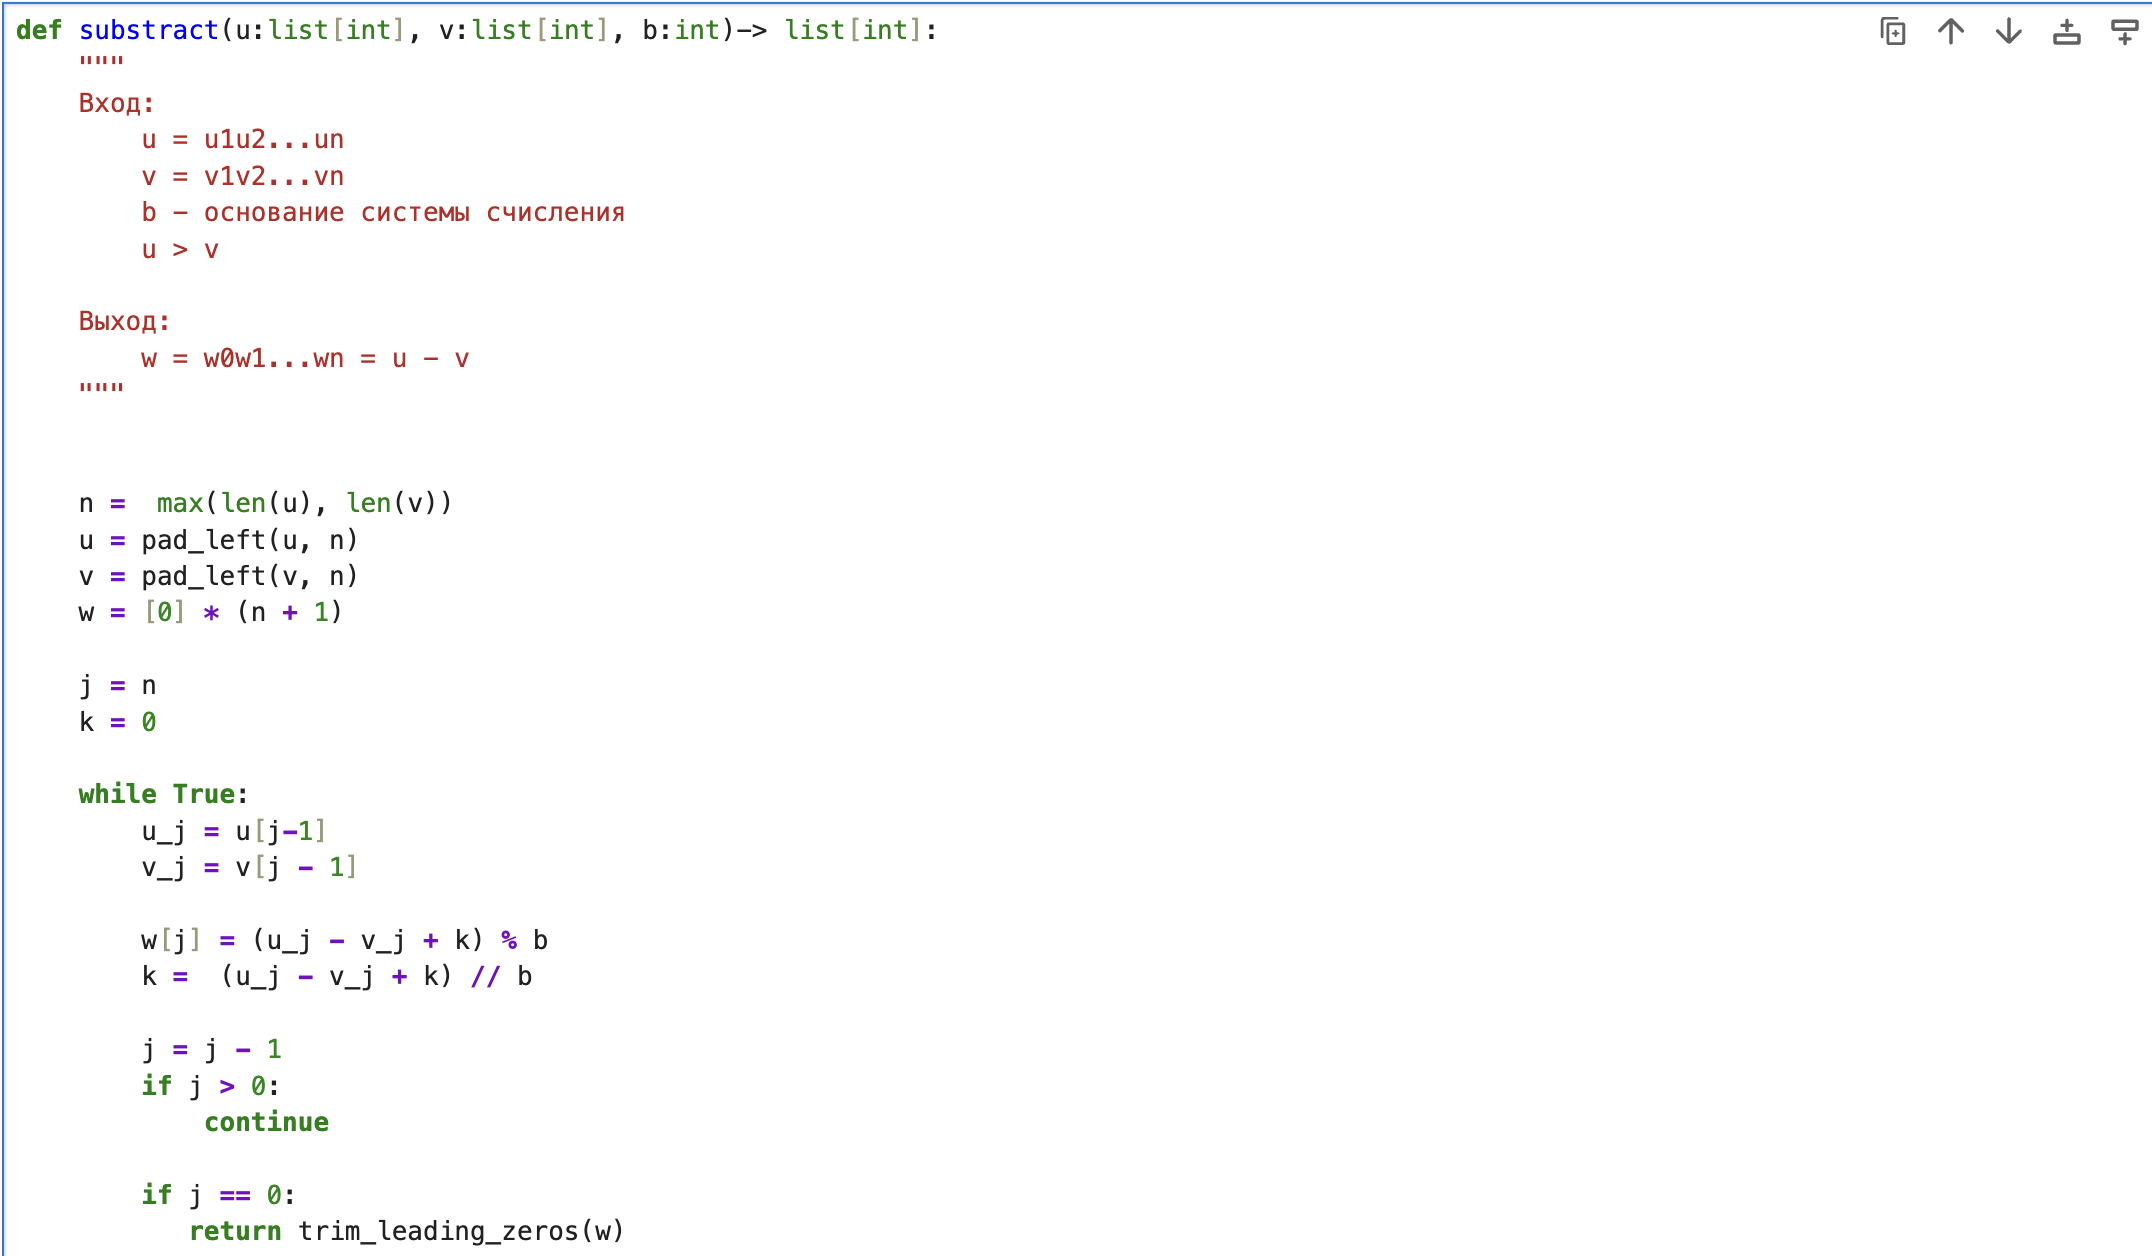
\includegraphics[keepaspectratio]{./image/img_11.png}}

}

\caption{substract}

\end{figure}%

\begin{figure}[H]

{\centering \pandocbounded{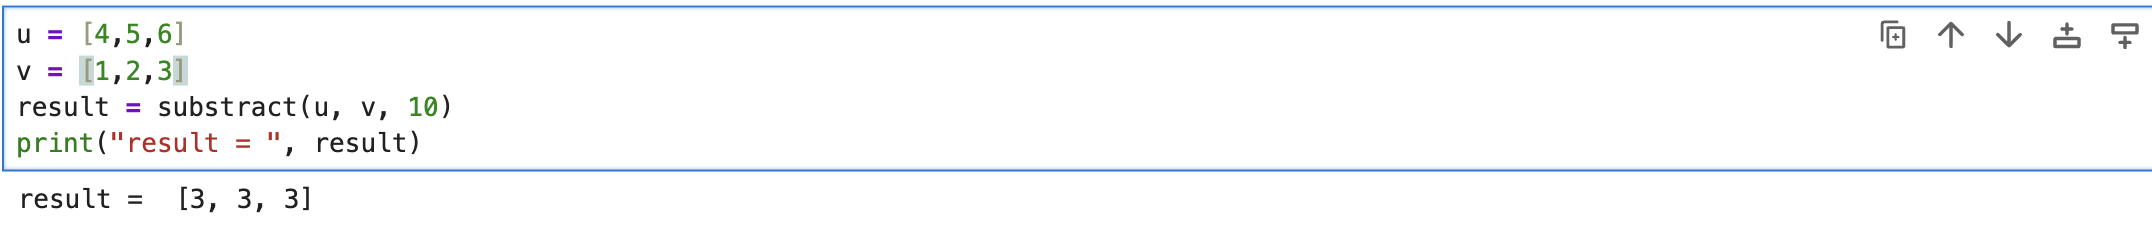
\includegraphics[keepaspectratio]{./image/img_10.png}}

}

\caption{result}

\end{figure}%

\section{Реализация Алгоритма умножения неотрицательных целых чисел
столбиком}\label{ux440ux435ux430ux43bux438ux437ux430ux446ux438ux44f-ux430ux43bux433ux43eux440ux438ux442ux43cux430-ux443ux43cux43dux43eux436ux435ux43dux438ux44f-ux43dux435ux43eux442ux440ux438ux446ux430ux442ux435ux43bux44cux43dux44bux445-ux446ux435ux43bux44bux445-ux447ux438ux441ux435ux43b-ux441ux442ux43eux43bux431ux438ux43aux43eux43c}

\begin{figure}[H]

{\centering \pandocbounded{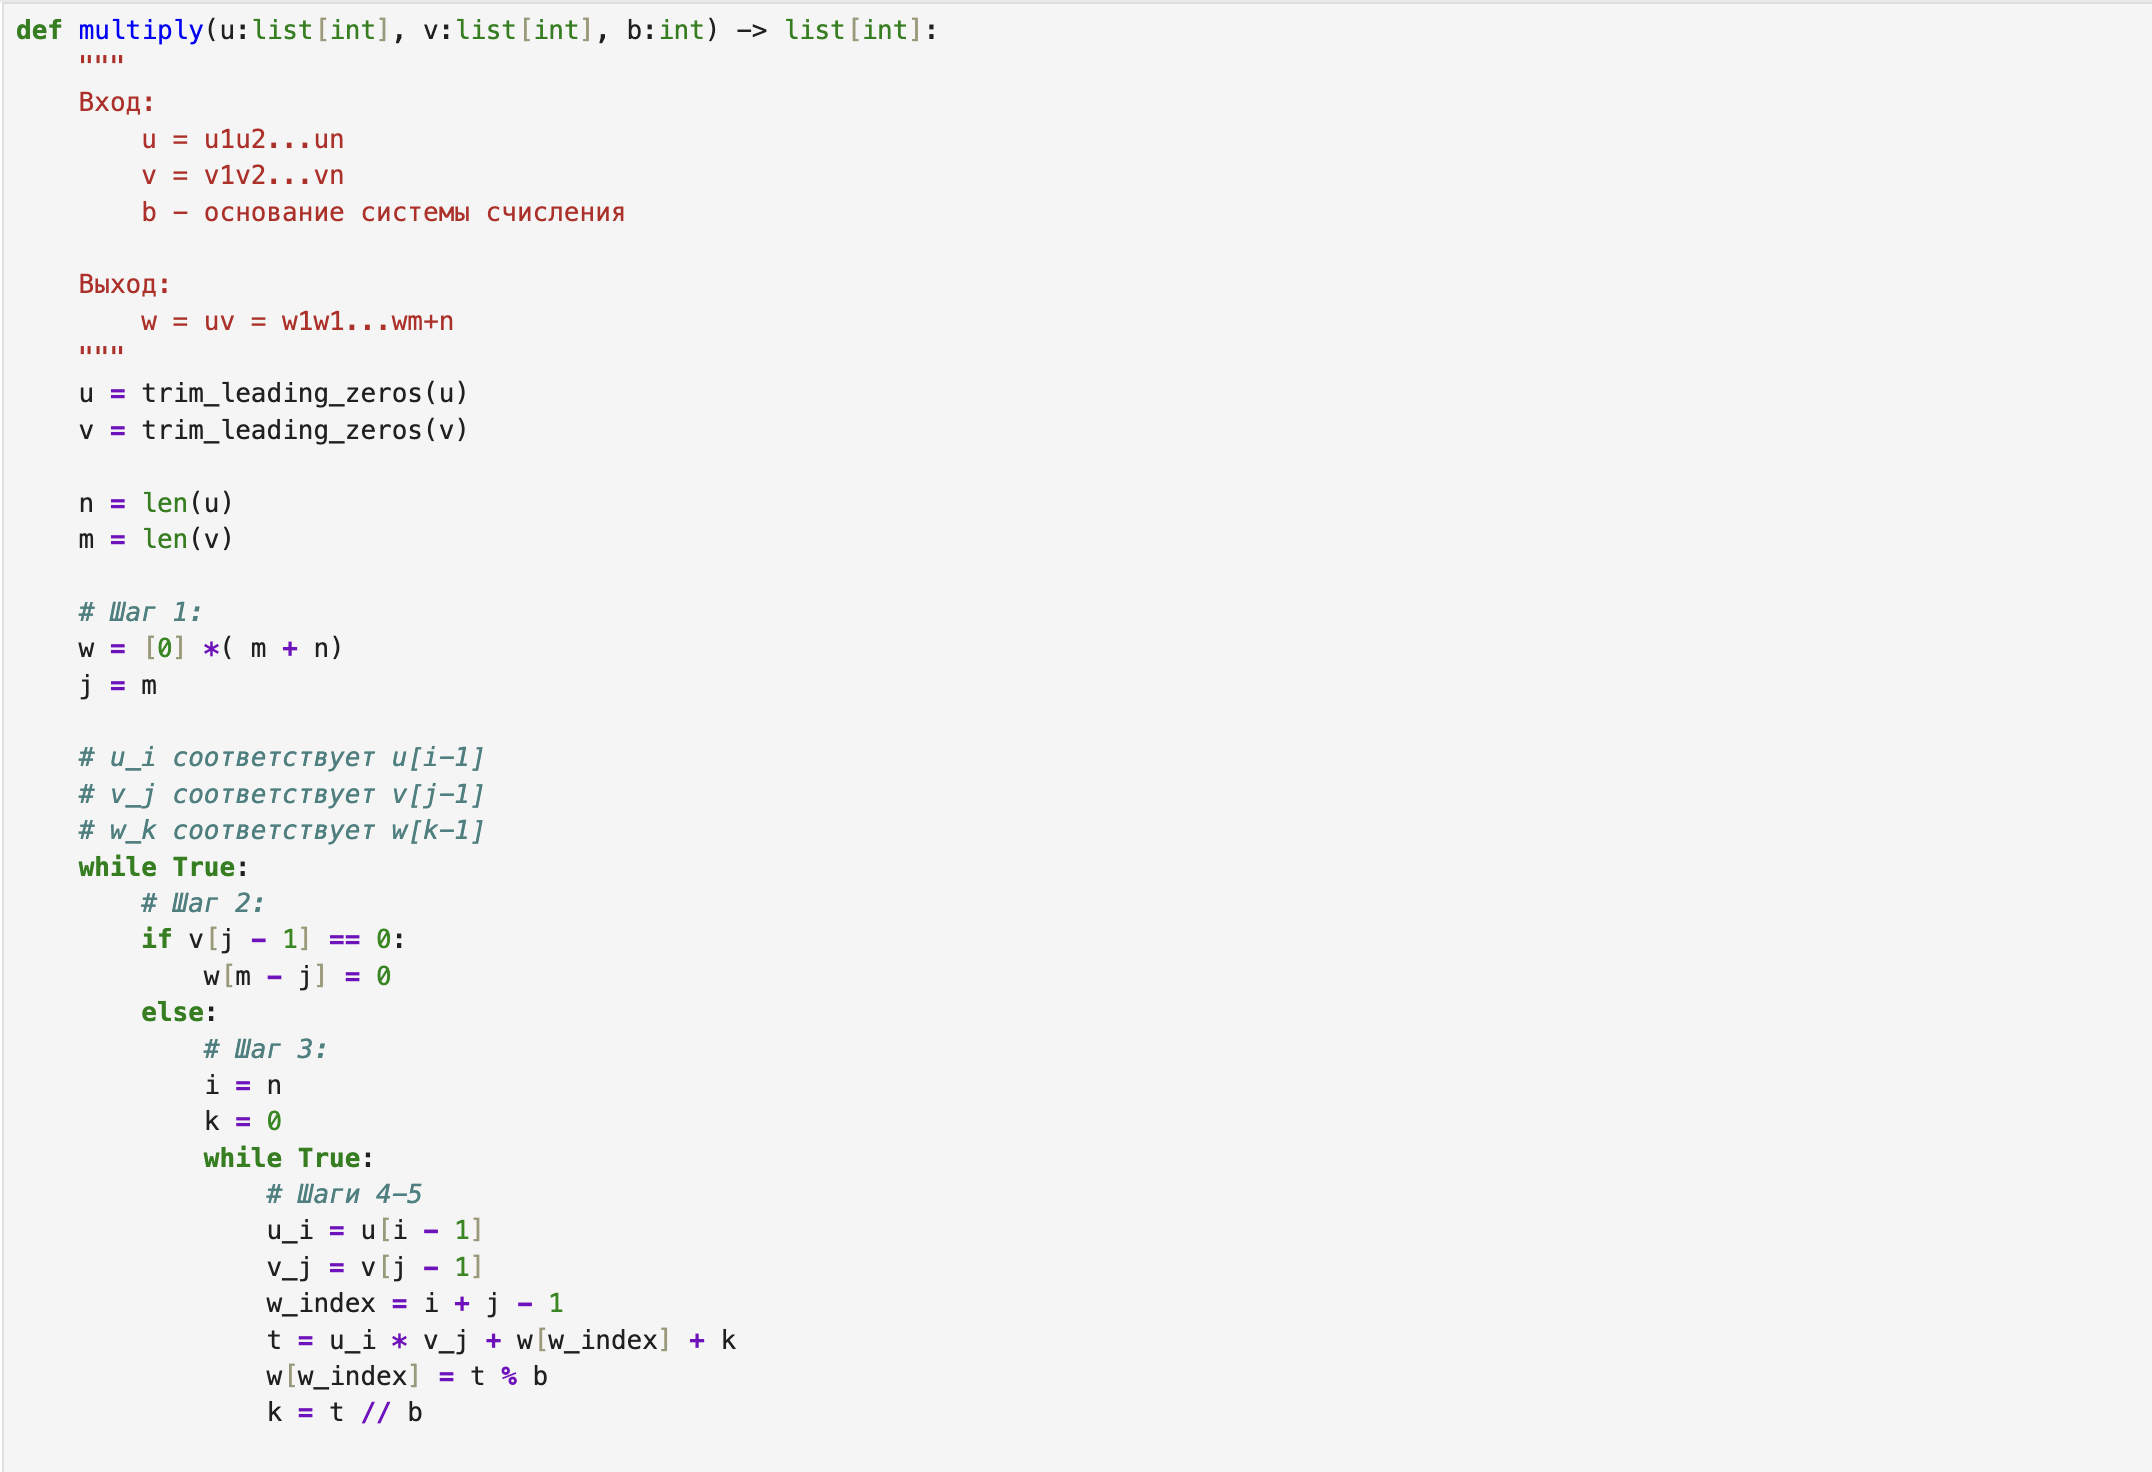
\includegraphics[keepaspectratio]{./image/img_9.png}}

}

\caption{multiply}

\end{figure}%

\begin{figure}[H]

{\centering \pandocbounded{
\includegraphics[keepaspectratio]{./image/img_8.png}}

}

\caption{multiply}

\end{figure}%

\begin{figure}[H]

{\centering \pandocbounded{
\includegraphics[keepaspectratio]{./image/img_7.png}}

}

\caption{result}

\end{figure}%

\section{Реализация Алгоритма умножения методом быстрого
столбика}\label{ux440ux435ux430ux43bux438ux437ux430ux446ux438ux44f-ux430ux43bux433ux43eux440ux438ux442ux43cux430-ux443ux43cux43dux43eux436ux435ux43dux438ux44f-ux43cux435ux442ux43eux434ux43eux43c-ux431ux44bux441ux442ux440ux43eux433ux43e-ux441ux442ux43eux43bux431ux438ux43aux430}

\begin{figure}[H]

{\centering \pandocbounded{
\includegraphics[keepaspectratio]{./image/img_6.png}}

}

\caption{multiply\_fast}

\end{figure}%

\begin{figure}[H]

{\centering \pandocbounded{
\includegraphics[keepaspectratio]{./image/img_5.png}}

}

\caption{result}

\end{figure}%

\section{Реализация Алгоритма деления неотрицательных целых
чисел}\label{ux440ux435ux430ux43bux438ux437ux430ux446ux438ux44f-ux430ux43bux433ux43eux440ux438ux442ux43cux430-ux434ux435ux43bux435ux43dux438ux44f-ux43dux435ux43eux442ux440ux438ux446ux430ux442ux435ux43bux44cux43dux44bux445-ux446ux435ux43bux44bux445-ux447ux438ux441ux435ux43b}

\begin{figure}[H]

{\centering \pandocbounded{
\includegraphics[keepaspectratio]{./image/img_4.png}}

}

\caption{helper functions}

\end{figure}%

\begin{figure}[H]

{\centering \pandocbounded{
\includegraphics[keepaspectratio]{./image/img_3.png}}

}

\caption{division}

\end{figure}%

\begin{figure}[H]

{\centering \pandocbounded{
\includegraphics[keepaspectratio]{./image/img_2.png}}

}

\caption{division}

\end{figure}%

\begin{figure}[H]

{\centering \pandocbounded{
\includegraphics[keepaspectratio]{./image/img_1.png}}

}

\caption{result}

\end{figure}%

\chapter{Выводы}\label{ux432ux44bux432ux43eux434ux44b}

Реализовал алгоритмов многократной точности для целочисленной
арифметики.

\chapter*{Список
литературы}\label{ux441ux43fux438ux441ux43eux43a-ux43bux438ux442ux435ux440ux430ux442ux443ux440ux44b}
\addcontentsline{toc}{chapter}{Список литературы}

https://en.wikipedia.org/wiki/Arbitrary-precision\_arithmetic


\printbibliography



\end{document}
